% !TEX program = pdflatex
% Paper 2: Orthogonality Screening of Topological Indices for QSPR Modeling
% Compile with: pdflatex paper2_orthogonality_screening.tex (twice for cross-refs)

\documentclass[11pt,a4paper]{article}

\usepackage[T1]{fontenc}
\usepackage[utf8]{inputenc}
\usepackage{lmodern}
\usepackage[margin=1in]{geometry}
\usepackage{amsmath,amssymb,amsthm}
\usepackage{mathtools}
\usepackage{booktabs}
\usepackage{array}
\usepackage{graphicx}
\graphicspath{{../figures/}}
\usepackage{hyperref}
\hypersetup{colorlinks=true,linkcolor=blue!50!black,citecolor=blue!50!black,urlcolor=blue!50!black}
\usepackage{xcolor}
\usepackage{enumitem}
\setlist[itemize]{topsep=2pt,itemsep=2pt}
\usepackage{listings}
\lstset{basicstyle=\ttfamily\small,frame=single,breaklines=true,xleftmargin=1em,xrightmargin=1em,numbers=none}

\newtheorem{theorem}{Theorem}[section]
\newtheorem{proposition}[theorem]{Proposition}
\newtheorem{lemma}[theorem]{Lemma}
\newtheorem{corollary}[theorem]{Corollary}
\theoremstyle{definition}
\newtheorem{definition}[theorem]{Definition}
\newtheorem{remark}[theorem]{Remark}

% \todo marker: suppressed (no draft markers remain in body).
\newcommand{\todo}[1]{}
\newcommand{\bid}{\mathcal{F}_{\mathrm{BID}}}

\title{\bfseries Orthogonality Screening of Topological Indices for QSPR Modeling:\\ A Structural and Empirical Redundancy Analysis}

\author{
  Ganesh Shiwakoti\thanks{Department of Mathematics and Statistics, Florida Atlantic University, USA. \texttt{ganshiwakoti@gmail.com}} \and
  Advik Natarajan\thanks{Department of Mathematics, Loyola College, Chennai, India.} \and
  Michael Arockiaraj\footnotemark[2]
}

\date{Draft of \today}

\begin{document}
\maketitle

\begin{abstract}
\textbf{Problem.} The chemical graph theory literature contains
many hundreds of scalar topological indices proposed for QSPR/QSAR
modelling, and the conventional pairwise-correlation criterion for
``does a new index carry independent information''
($\max_{b} \lvert r(z, X_b)\rvert < 0.95$ against a classical
baseline) is empirically over-permissive.

\textbf{Method.} We present an open-source diagnostic pipeline
combining four standard diagnostics --- pairwise correlation, PCA
effective rank, variance inflation factor, and partial correlation
with the QSPR target --- into a single \emph{combined diagnostic}
(Table~\ref{tab:decision}), positioned as a \emph{conservative
pre-flight screen for independent linear QSPR signal}, not as a
hard feature-selection filter or a QSPR-utility certification. The
\emph{Edge-Degree-Pair Basis} (Theorem~\ref{thm:bid}) gives a
complementary structural ceiling: every bond-incident-degree (BID)
index on hydrogen-suppressed molecular graphs with maximum degree
$\Delta \le 4$ lies in a vector space of dimension at most
$\binom{5}{2} = 10$.

\textbf{Evidence.} Across three regression QSPR datasets (ESOL,
FreeSolv, Lipophilicity; $n = 5\,966$ molecules in total), the
three-parameter Wuzi index family of the companion
paper~\cite{Paper1_Wuzi} fails the combined diagnostic at every
one of the $300$ grid points sampled, and the qualitative verdict
is stable across the nine $(\tau_r, \tau_{\mathrm{pcor}})$
combinations in $\{0.90, 0.95, 0.99\} \times \{0.05, 0.10, 0.20\}$
(\S\ref{sub:threshold_sensitivity}). A cross-dataset replication on
$20$ alternative-family candidates (information-theoretic,
centrality, motif, eccentricity, spectral-hybrid) over all four
benchmarks shows that $15$--$17/20$ clear the pairwise threshold
but only $0$--$4/20$ also clear
$\lvert\mathrm{pcor}(z, y \mid X)\rvert \ge 0.10$: pairwise-only
screening is uniformly over-permissive, and the combined diagnostic
is even more selective on FreeSolv, Lipophilicity, and BBBP than on
ESOL (Table~\ref{tab:novel_combined}). A 5-fold cross-validated
RandomForest benchmark on those four datasets shows the
pairwise-pruned feature set preserves predictive performance within
CV noise at roughly $4\times$ fewer features
(Table~\ref{tab:ml_benchmark}), and matches or beats LASSO,
ElasticNet, mRMR, Boruta, and L1-logistic feature-selection
comparators on every dataset (Table~\ref{tab:fs_comparison}).

\textbf{Limitation.} On Lipophilicity the strict combined
diagnostic retains zero features in $4/5$ ML-benchmark folds; the
combined diagnostic should be read as evidence about residual
target signal, \emph{not} as an automatic feature-selection rule.
We do not claim universal QSPR usefulness of the pipeline,
universal redundancy of the Wuzi family beyond the tested datasets
and linear diagnostics, or chemical utility of any alternative-family
candidate that clears the combined diagnostic on a single dataset;
full limitations are catalogued in \S\ref{sub:limitations}.

\medskip
\noindent\textbf{Keywords.} Topological index, orthogonality
screening, redundancy analysis, QSPR, principal component analysis,
partial correlation, bond-incident-degree (BID) family.

\medskip
\noindent\textbf{Code and data.}
\url{https://github.com/Singati2/topological-index-orthogonality}
\end{abstract}

% =====================================================================
\section{Introduction}
% =====================================================================

The vocabulary of scalar topological indices used in QSPR/QSAR
modeling has grown over six decades from a handful of
proposals \cite{Wiener1947, Randic1975, Gutman1972} to several
hundred. Many indices are interrelated by exact identity (e.g.\
the harmonic index $H$ is $2$ times the special case
$\beta=-1$ of the general sum-connectivity index $\chi_\beta$), and
in practice the empirical Pearson correlations between proposed
indices on a fixed dataset can exceed $|r|=0.95$ for the majority
of pairs.

This raises a recurring methodological question. \emph{What does a
newly proposed scalar topological index need to demonstrate to be
treated as a meaningful contribution to QSPR modeling?} Three
weak forms of justification appear frequently in the literature:
\begin{enumerate}[label=(\roman*)]
\item Strong correlation with a chemical property on a small dataset
(e.g.\ $18$ octanes, $75$ decanes), often without reference to a
classical-baseline comparison.
\item A closed-form value on standard graph classes, framed as
mathematical novelty.
\item Parametric generality (a new parameter that subsumes the
classical case at one specific parameter value).
\end{enumerate}
None of these by themselves is sufficient to demonstrate
\emph{independent} predictive value beyond the classical baseline.

This paper proposes an explicit pre-flight check for the
``does it carry independent information'' question, framed
operationally so that any author can apply it.

\subsection{Contributions}

\begin{enumerate}[label=(\arabic*)]
\item An open-source orthogonality-screening pipeline
(Section~\ref{sec:protocol}) covering correlation matrix,
PCA, VIF, and partial correlation with the QSPR target, using
a fixed redundancy threshold $|r|\ge 0.95$.
\item Replication across three independent MoleculeNet
benchmarks (Section~\ref{sec:datasets}).
\item A structural observation (Section~\ref{sec:bid}, the
\emph{Edge-Degree-Pair Basis}) giving a dimension-$10$ ceiling on
the BID family on $\mathcal{G}_4$ (hydrogen-suppressed molecular
graphs).
\item Two case studies: the parametric Wuzi index family
(Section~\ref{sec:wuzi_case}, $300$ grid points) and twenty
alternative-family candidate indices
(Section~\ref{sec:novel_case}).
\item Explicit positioning of orthogonality as \emph{necessary but
not sufficient} for QSPR usefulness, with empirical evidence
(Section~\ref{sec:discussion}).
\end{enumerate}

% =====================================================================
\section{Related work}\label{sec:related}
% =====================================================================

\subsection{Relation to the companion graph-theory paper}\label{sec:relation_companion}

The mathematical-chemistry properties of the Wuzi index family ---
its definition, closed-form values on standard graph classes,
bracket and ratio bounds, Cauchy--Schwarz and Jensen-type bounds
in $M_1$, $M_2$, $R$, $\chi$, and $SO$, the empirical
extremal-graph pattern (including the spider / double-spider
structural conjecture at the mixed-sign triple
$(\alpha, \beta, \gamma) = (-1, -1, 1)$ verified through tree
order $n = 20$), and sensitivity-analysis benchmarks on $18$
octanes, $106$ trees of order $10$, and $75$ decane isomers ---
are developed in a companion graph-theory
paper~\cite{Paper1_Wuzi}. The present paper is focused on the
screening pipeline as a reusable methodology and uses the Wuzi
family only as one screened candidate (Section~\ref{sec:wuzi_case}),
re-deriving no Wuzi-specific mathematical results. A reader
interested only in the screening methodology can treat the Wuzi
family as a black-box parametric BID family throughout.

\subsection{Orthogonality and redundancy of topological indices}

The recognition that many topological indices are mutually highly
correlated is not new. \cite{MovahediGutmanRedzepovicFurtula2026}
Section~5.2 includes an intercorrelation analysis among
Sombor-family variants showing pairwise $r$-values above $0.9$ on
the octane data. Other intercorrelation observations appear
sporadically in the BID-bounds literature. The present work
extends this style of observation in three ways: (i)~by fixing a
threshold $|r|\ge 0.95$ and applying it uniformly across datasets;
(ii)~by replicating across three independent QSPR benchmarks rather
than a single small dataset; and (iii)~by combining
PCA, partial correlation, and VIF with the pairwise correlation
analysis to assess different aspects of redundancy.

\subsection{The bond-incident-degree (BID) family}

\emph{Bond-incident-degree} (BID) indices are functionals of the
form $I_f(G)=\sum_{uv\in E(G)} f(d_u,d_v)$ for a symmetric
function $f$. This unifies the bulk of the classical degree-based
topological-index literature: Zagreb $M_1,M_2$, modified Zagreb,
forgotten $F$, Randi\'c $R$ and general $R_\alpha$,
sum-connectivity $\chi$ and general $\chi_\beta$, harmonic $H$,
the geometric--arithmetic index $GA$ of Vuki\v{c}evi\'c and
Furtula~\cite{VukicevicFurtula2009GA}, arithmetic-geometric $AG$,
atom-bond connectivity $ABC$, augmented Zagreb $AZI$, Sombor $SO$
and its variants, the Albertson irregularity index
$\mathrm{Alb}$~\cite{Albertson1997}, sigma $\sigma$, and reduced
Zagreb $\mathrm{redM}_1$. The observation that BID
indices are linear functionals of the edge-degree-pair counts
$m_{ij}$ is standard~\cite{BorovicaninDasFurtulaGutman2017Zagreb}; what we
contribute is the explicit dimension bound on $\mathcal{G}_4$ and
the redundancy-screening consequence.

\subsection{QSPR benchmarks and reproducibility}

The QSPR benchmarks used here (ESOL, FreeSolv, Lipophilicity) are
drawn from the MoleculeNet collection~\cite{MoleculeNet}, a
standard reference for molecular property prediction. We use the
versions distributed via MoleculeNet without resplitting; SMILES
are processed through RDKit~\cite{RDKit} and converted to
hydrogen-suppressed molecular graphs through a thin NetworkX
wrapper.

\subsection{Relation to generic feature-selection methods}\label{sec:feature_selection}

The broader cheminformatics descriptor-redundancy literature is
documented in the Todeschini--Consonni
handbook~\cite{TodeschiniConsonniHandbook}, which catalogues the
classical molecular-descriptor families and the standard pairwise
and multivariate redundancy diagnostics. Outside cheminformatics,
generic feature-selection methods --- the minimum-redundancy
maximum-relevance criterion (mRMR)~\cite{PengLongDing2005},
the Boruta wrapper~\cite{KursaRudnicki2010}, and embedded
methods such as LASSO~\cite{Tibshirani1996} --- select features
from an arbitrary descriptor matrix conditional on a fixed target
and model class.

The present pipeline is positioned at a different layer in the
modelling stack. The pairwise / PCA / VIF diagnostics are
\emph{target-agnostic}; the partial-correlation step is
\emph{target-aware but model-agnostic}; and the combined diagnostic
is designed as a \emph{pre-flight check for a single proposed new
topological index} against a fixed classical baseline, not as a
competitor for end-to-end QSPR feature selection. Conceptually,
the two layers compose rather than compete: the screening pipeline
gates which indices enter the descriptor matrix, after which
mRMR / LASSO / Boruta / similar methods could be applied
downstream to the screened set against the modelling task at hand.
Comparing redundancy-screening pipelines against generic
feature-selection benchmarks on a full QSPR endpoint is outside
the scope of the present paper and is noted as future work in
Section~\ref{sec:discussion}.

% =====================================================================
\section{Datasets and implementation}\label{sec:datasets}
% =====================================================================

\begin{table}[h]
\centering
\caption{QSPR benchmark datasets used in this study.}
\label{tab:datasets}
\begin{tabular}{llrl}
\toprule
Name & Target property & $n$ & Source\\
\midrule
ESOL          & $\log S$ (aqueous solubility, mol/L) & $1\,127$ & \cite{Delaney2004ESOL} via \cite{MoleculeNet}\\
FreeSolv      & $\Delta G_{\mathrm{hyd}}$ (hydration free energy, kcal/mol) & $639$ & \cite{Mobley2014FreeSolv} via \cite{MoleculeNet}\\
Lipophilicity & $\log D$ at pH 7.4 & $4\,200$ & \cite{LipophilicityChEMBL} via \cite{MoleculeNet}\\
\bottomrule
\end{tabular}
\end{table}

The $30$-index classical baseline (Table~\ref{tab:baseline}) is
implemented in the reference codebase
(\texttt{src/standard\_indices.py}); each index admits a $\le 20$-line
Python implementation, and the full $30$-index computation for a
single graph takes a few milliseconds. The reference
implementation is open-source under MIT license.

\begin{table}[h]
\centering
\caption{$30$-index classical baseline used for orthogonality screening.}
\label{tab:baseline}
\small
\begin{tabular}{ll}
\toprule
Family & Indices\\
\midrule
Degree-based (18) & $M_1$, $M_2$, $mM_1$, $mM_2$, $F$, $R$, SCI, $H$, $GA$, $AG$, ABC, ABS, AZI, $SO$, $SO_{\mathrm{red}}$, Alb, $\sigma$, $\mathrm{redM}_1$\\
Distance-based (8) & $W$, WW, HR, MTI (Schultz), Gutman, Mostar, $Sz$, $PI$\\
Spectral (3) & EE, Energy, Spectral Radius\\
Other (1) & Balaban $J$\\
\bottomrule
\end{tabular}
\end{table}

% =====================================================================
\section{The Edge-Degree-Pair Basis observation}\label{sec:bid}
% =====================================================================

We isolate a structural reason why the BID family on
hydrogen-suppressed molecular graphs is redundancy-prone. The
theorem is restated here for completeness because it is used
\emph{operationally} in the screening argument (in particular, as
the structural upper bound that licenses the redundancy
verdict on the Wuzi family in
Section~\ref{sec:wuzi_case}); the same theorem appears in the
companion graph-theory paper~\cite{Paper1_Wuzi}, where it sets
the structural ceiling for the Wuzi-specific mathematical
consequences. The novelty in the present paper is not the theorem
itself --- the linearity observation that underpins it is standard
in the mathematical-chemistry literature~\cite{BorovicaninDasFurtulaGutman2017Zagreb}
--- but its operational use inside the screening pipeline.

\begin{theorem}[Edge-Degree-Pair Basis]\label{thm:bid}
Let $\mathcal{G}_\Delta$ denote the class of finite simple graphs
with maximum degree at most $\Delta$. For any BID index
$I_f\in\bid$ and any $G\in\mathcal{G}_\Delta$,
\begin{equation}\label{eq:bid_linear}
I_f(G)=\sum_{1\le i\le j\le\Delta} f(i,j)\cdot m_{ij}(G),
\end{equation}
where $m_{ij}(G)=\bigl|\{uv\in E(G):\{d_u,d_v\}=\{i,j\}\}\bigr|$.
Restricted to $\mathcal{G}_4$, the vector space spanned by all BID
indices has dimension at most $\binom{4+1}{2}=10$.
\end{theorem}

\begin{proof}
We establish the linear-decomposition identity~\eqref{eq:bid_linear}
first and then deduce the dimension bound.

\emph{Step 1: linear decomposition.} Fix $G\in\mathcal{G}_\Delta$ and,
for each pair $(i,j)$ with $1\le i\le j\le\Delta$, define
$E_{ij}(G) = \{ uv\in E(G) \,:\, \{d_u,d_v\}=\{i,j\}\}$,
so that $m_{ij}(G)=|E_{ij}(G)|$. Because every edge has
$d_u,d_v\in\{1,\ldots,\Delta\}$, the family $\{E_{ij}(G)\}_{i\le j}$
partitions $E(G)$. Hence
\[
I_f(G) = \sum_{uv\in E(G)} f(d_u,d_v)
= \sum_{1\le i\le j\le\Delta}\;\sum_{uv\in E_{ij}(G)} f(d_u,d_v).
\]
For every $uv\in E_{ij}(G)$ the multiset $\{d_u,d_v\}$ equals
$\{i,j\}$ and $f$ is symmetric, so $f(d_u,d_v)=f(i,j)$ is constant
on the inner sum, which collapses to $f(i,j)\cdot m_{ij}(G)$ and
yields~\eqref{eq:bid_linear}.

\emph{Step 2: dimension bound.} For each admissible pair $(i,j)$
with $1\le i\le j\le\Delta$, regard the edge-count
$m_{ij}:\mathcal{G}_\Delta\to\mathbb{N}_{\ge 0}$ as a functional on
$\mathcal{G}_\Delta$. Equation~\eqref{eq:bid_linear} shows
$I_f = \sum_{i\le j} f(i,j)\cdot m_{ij}$ as functionals on
$\mathcal{G}_\Delta$, so
$\bid \subseteq \operatorname{span}_{\mathbb{R}}\{m_{ij}:1\le i\le j\le\Delta\}$.
A subspace of a span of $N_\Delta$ vectors has dimension at most
$N_\Delta$, hence
$\dim_{\mathbb{R}}\bid \le N_\Delta = \binom{\Delta+1}{2}$ by the
standard multiset-counting identity. For $\Delta=4$ this is
$\binom{5}{2}=10$.
\end{proof}

\begin{remark}\label{rem:bid_credit}
The observation that BID indices are linear in $m_{ij}$ counts is
standard~\cite{BorovicaninDasFurtulaGutman2017Zagreb}. The contribution here is
(i)~the explicit dimension-$10$ bound on $\mathcal{G}_4$ and
(ii)~its operational use in the screening pipeline: any new BID
index proposed for molecular chemistry must justify its
independence from the existing zoo within a $10$-dimensional
subspace.
\end{remark}

\begin{corollary}\label{cor:bid_redundancy}
On $\mathcal{G}_4$, any $11$ BID indices are linearly dependent.
Parametric BID families (general Randi\'c $R_\alpha$, general
sum-connectivity $\chi_\beta$, Wuzi, etc.) cannot escape the
$10$-dimensional ceiling by adding parameters.
\end{corollary}

In practice, the rank of the matrix $M$ with rows
$(m_{11}, m_{12}, \ldots, m_{44})$ over a chemistry dataset is
strictly less than $10$ because several $m_{ij}$ are sparse or
near-constant. For example, $m_{14}$ and $m_{44}$ require
quaternary carbons connected to methyl groups (rare),
$m_{11}$ requires an isolated bond (extremely rare in drug-like
chemistry).

% =====================================================================
\section{The screening protocol}\label{sec:protocol}
% =====================================================================

Let $X\in\mathbb{R}^{n\times p}$ be a matrix of $p$ baseline indices
on $n$ molecules, $y\in\mathbb{R}^n$ the target property, and
$z\in\mathbb{R}^n$ the candidate index values on the same molecules.
The screening pipeline produces four diagnostics.

\subsection{Pairwise correlation and redundancy threshold}
Compute the $p\times p$ Pearson correlation matrix $\mathrm{Cor}(X)$
and the vector of correlations $\mathrm{cor}(z,X_b)$ for
$b=1,\ldots,p$. The candidate is \emph{statistically redundant} if
$\max_b|\mathrm{cor}(z,X_b)|\ge\tau$ for a threshold $\tau$ (we
report $\tau=0.95$ as the primary threshold and also
$\tau=0.90$ as a secondary check). The redundant-pair count
inside the baseline,
$|\{(b_1,b_2):|\mathrm{Cor}(X)_{b_1,b_2}|\ge\tau\}|$, is a
companion summary statistic of baseline redundancy.

\subsection{Principal-component effective rank}
Compute the PCA of the standardized baseline $X$. Let
$\lambda_1\ge\lambda_2\ge\cdots\ge\lambda_p$ be the eigenvalues of
$\mathrm{Cor}(X)$ and $C_k=\sum_{i\le k}\lambda_i/\sum_i\lambda_i$
the cumulative variance fraction. The
$\mathrm{PC}_{1-\alpha}$ effective rank is the smallest $k$ with
$C_k\ge 1-\alpha$; we report $\mathrm{PC}_{95}, \mathrm{PC}_{99}$.

\subsection{Variance Inflation Factor}
For each baseline index $b$, $\mathrm{VIF}_b=(1-R_b^2)^{-1}$ where
$R_b^2$ is the coefficient of determination of $X_b$ regressed on
the other $p-1$ baseline columns. $\mathrm{VIF}_b>10$ is the
conventional ``high collinearity'' threshold;
$\mathrm{VIF}_b=\infty$ indicates exact linear dependence within
the baseline.

\subsection{Partial correlation with target}
Compute $z^{\mathrm{res}}=z-\hat z$ and $y^{\mathrm{res}}=y-\hat y$
where $\hat z, \hat y$ are the OLS fits regressing $z$ and $y$ on
the baseline $X$. The partial correlation
$\mathrm{pcor}(z,y\mid X)=\mathrm{cor}(z^{\mathrm{res}},y^{\mathrm{res}})$
measures the signal in $z$ relative to the target $y$ \emph{after}
controlling for everything the baseline already captures. We use
$|\mathrm{pcor}|<0.10$ as the conventional ``negligible
additional signal'' band.

\subsection{Decision summary}

\begin{table}[h]
\centering
\caption{Screening pipeline decision summary. Both conditions must hold for the candidate to be flagged as adding meaningful QSPR signal.}
\label{tab:decision}
\begin{tabular}{lll}
\toprule
Diagnostic & Pass condition & Interpretation\\
\midrule
$\max_b|\mathrm{cor}(z,X_b)|$ & $<\tau=0.95$ & not statistically redundant with the baseline\\
$|\mathrm{pcor}(z,y\mid X)|$  & $\ge 0.10$  & adds non-negligible target-relevant signal\\
\bottomrule
\end{tabular}
\end{table}

The combined diagnostic of Table~\ref{tab:decision} should be read
as a \emph{conservative pre-flight diagnostic for independent linear
QSPR signal}, not as a hard feature-selection filter or a utility
certification. Passing the screen does not prove utility; failing
the screen is evidence of redundancy under the tested baseline,
dataset, and linear diagnostics. We deliberately avoid language
such as ``meaningful new index'' in favour of the more precise
``candidate with non-negligible residual linear signal under the
tested $30$-index baseline''. Threshold sensitivity is documented
in \S\ref{sub:threshold_sensitivity} and the Lipophilicity failure
mode --- where the strict combined diagnostic retains zero features
in $4/5$ ML-benchmark folds --- is treated as a formal limitation
in \S\ref{sub:limitations}.

% =====================================================================
\section{Results}\label{sec:results}
% =====================================================================

The two case studies and the downstream cross-validated ML
benchmark together establish that (i) the Wuzi parametric BID
family is fully redundant against the classical baseline on every
QSPR dataset we tested (Section~\ref{sec:wuzi_case}); (ii) the
pairwise $|r| < 0.95$ screen is over-permissive when applied to
candidates from non-BID design families
(Section~\ref{sec:novel_case}); and (iii) the pairwise screen
preserves predictive performance within cross-validation noise on
four MoleculeNet benchmarks (Section~\ref{sec:ml_benchmark}). All
three results are reproducible from the public repository, and
the full per-dataset numerical tables are in
\texttt{results/}.

\subsection{Case study 1: the Wuzi parametric family}\label{sec:wuzi_case}

The Wuzi index family is the three-parameter BID family
$W(G;\alpha,\beta,\gamma) = \sum_{uv\in E(G)} (d_u d_v)^\alpha (d_u + d_v)^\beta
\exp(\gamma\cdot|d_u-d_v|/(d_u+d_v))$ developed in the companion
paper~\cite{Paper1_Wuzi}; we treat it here as one parametric BID
candidate and screen it on a $100$-point grid
$(\alpha, \beta, \gamma) \in \{-1, -1/2, 0, 1/2, 1\}^2 \times \{0, 1/2, 1, 2\}$
on each of the three regression QSPR datasets.

\subsubsection{Baseline redundancy on the three datasets}

\begin{table}[h]
\centering
\small
\caption{Baseline redundancy across the three QSPR datasets. Pair counts are out of $\binom{30}{2}=435$. $\mathrm{PC}_{\alpha}$ is the smallest number of principal components whose cumulative explained variance is at least $\alpha\%$ of the baseline.}
\label{tab:baseline_redundancy}
\begin{tabular}{lrrrrrr}
\toprule
Dataset & $n$ & $\lvert r\rvert \ge 0.90$ & $\lvert r\rvert \ge 0.95$ & $\mathrm{PC}_{90}$ & $\mathrm{PC}_{95}$ & $\mathrm{PC}_{99}$\\
\midrule
ESOL          & $1127$ & $203$ ($46.7\%$) & $159$ ($36.6\%$) & $2$ & $3$ & $5$\\
FreeSolv      & $\phantom{0}639$ & $257$ ($59.1\%$) & $162$ ($37.2\%$) & $2$ & $3$ & $5$\\
Lipophilicity & $4200$ & $200$ ($46.0\%$) & $164$ ($37.7\%$) & $2$ & $3$ & $5$\\
\bottomrule
\end{tabular}
\end{table}

Across three independent datasets the pattern is consistent: about
$37\%$ of the $435$ baseline pairs are above the $0.95$ threshold,
and three principal components capture $95\%$ of the variance
(Figs.~\ref{fig:pca},~\ref{fig:redundancy_bars}).
Figure~\ref{fig:corr_heatmap} shows the full
$30 \times 30$ baseline correlation matrix on ESOL; the dense red
block in the upper-left corner is the degree-based index family,
which drives most of the redundancy reported in
Table~\ref{tab:baseline_redundancy}.

\begin{figure}[h]
\centering
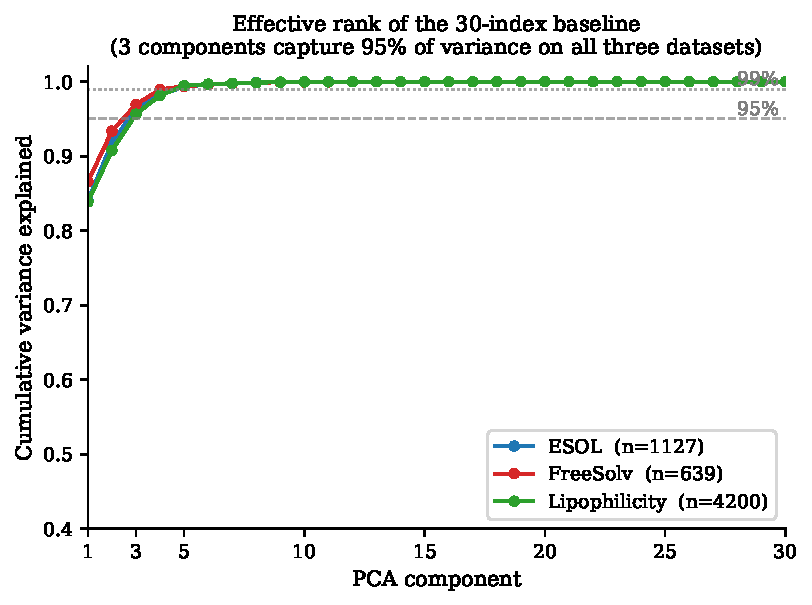
\includegraphics[width=0.75\linewidth]{fig2_pca_scree.pdf}
\caption{Cumulative explained variance of PCA on the $30$-index baseline.}
\label{fig:pca}
\end{figure}

\begin{figure}[h]
\centering
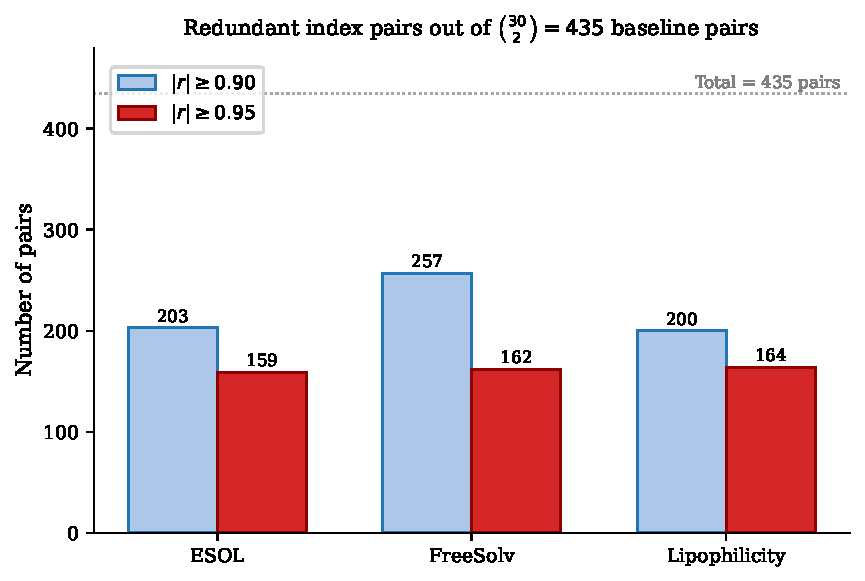
\includegraphics[width=0.65\linewidth]{fig3_redundancy_bars.pdf}
\caption{Redundant index-pair counts out of $\binom{30}{2}=435$ baseline pairs at two thresholds.}
\label{fig:redundancy_bars}
\end{figure}

\begin{figure}[h]
\centering
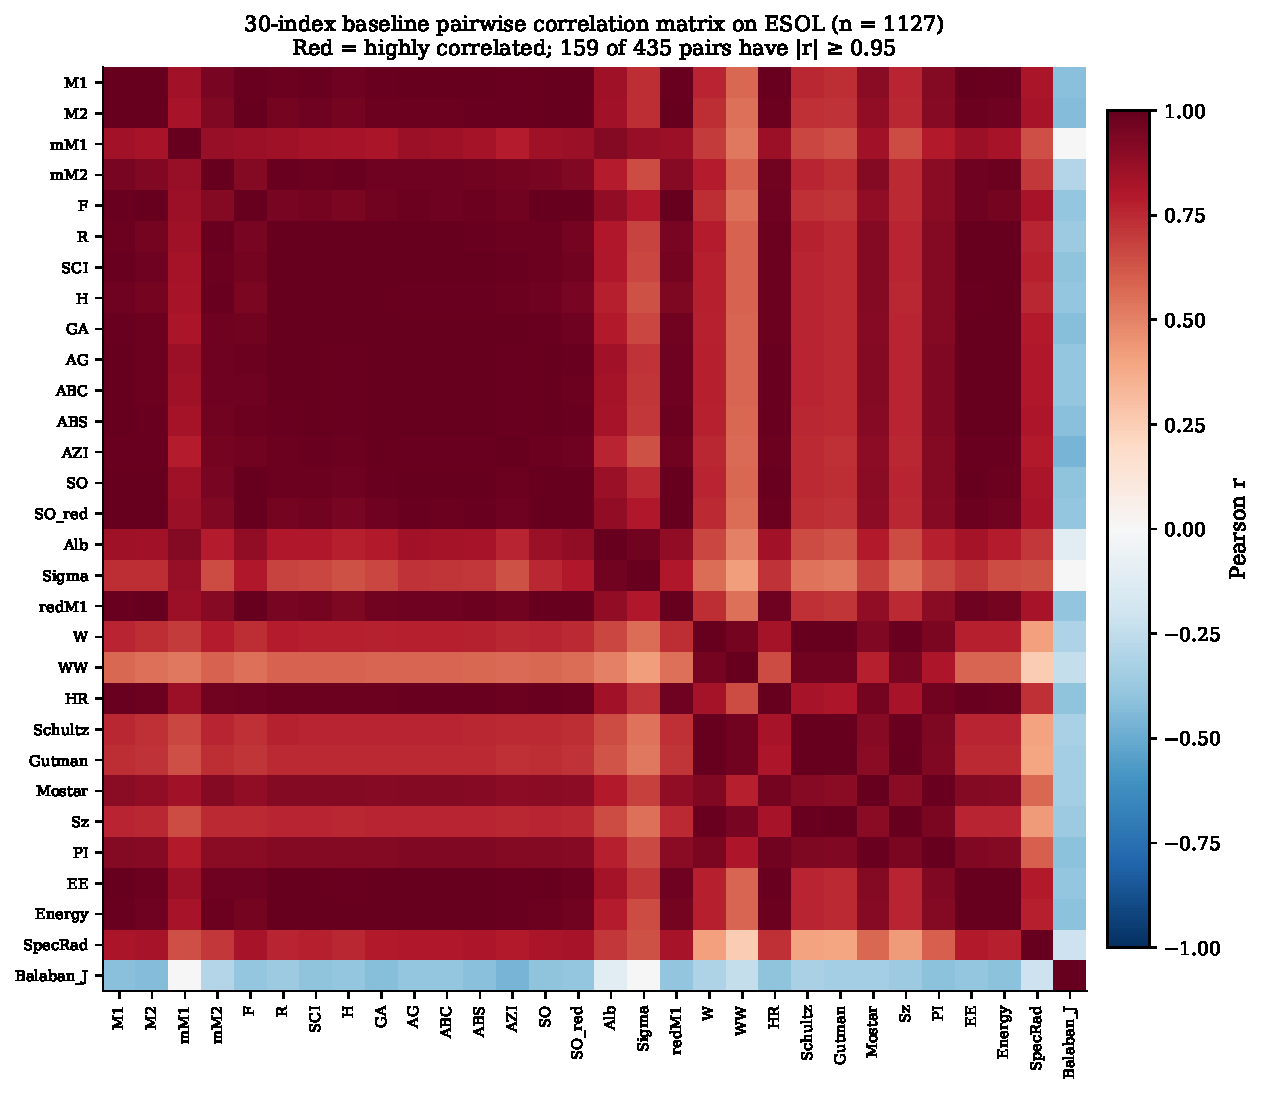
\includegraphics[width=0.6\linewidth]{fig8_correlation_heatmap.pdf}
\caption{$30\times 30$ baseline correlation matrix on ESOL. The dense red core is the degree-based index block.}
\label{fig:corr_heatmap}
\end{figure}

\subsubsection{Wuzi-family screening verdict and the multi-dimensional redundancy at $(-1,-1,1)$}

We screen the Wuzi family on $100$ grid points per dataset
($300$ grid points across the three QSPR datasets) and report the
compact per-dataset verdict in Table~\ref{tab:wuzi_verdict_paper1}.
We isolate the parameter triple
$(\alpha, \beta, \gamma) = (-1, -1, 1)$ below because it is the
single methodologically central grid point of the entire sweep
and illustrates the necessary-but-not-sufficient nature of the
pairwise screen.

\begin{table}[h]
\centering
\small
\caption{Wuzi $100$-point grid screening verdict across three QSPR datasets. ``Pass'' counts grid points at which $\max_{b}\lvert r(W, X_b)\rvert$ is strictly below $0.95$ for every classical baseline index $X_b$. ``Min $\max\lvert r\rvert$'' is the across-grid minimum of $\max_b\lvert r\rvert$ (the best-passing grid point). ``Max $\lvert\mathrm{pcor}\rvert$'' is the across-grid maximum of $\lvert\mathrm{pcor}(W, y \mid X)\rvert$, the partial correlation of $W$ with the QSPR target $y$ after regressing $W$ on the $30$-index baseline $X$.}
\label{tab:wuzi_verdict_paper1}
\begin{tabular}{lcccc}
\toprule
Dataset & Pass (max $\lvert r\rvert < 0.95$) & Fail & Min max $\lvert r\rvert$ & Max $\lvert\mathrm{pcor}(W, y \mid X)\rvert$\\
\midrule
ESOL          & 0 & 100 & $0.965$ & $0.028$\\
FreeSolv      & 1 &  99 & $0.943$ & $0.036$\\
Lipophilicity & 0 & 100 & $0.965$ & $0.009$\\
\bottomrule
\end{tabular}
\end{table}

\textbf{Verdict.} Across the $300$ grid points the Wuzi family
clears the pairwise $\max|r| < 0.95$ screen at exactly one grid
point (FreeSolv at $(-1, -1, 1)$, $\max|r| = 0.943$ with $mM_2$).
The maximum partial correlation with the target across the $300$
grid points is $0.036$ (FreeSolv); the corresponding maxima on
ESOL and Lipophilicity are $0.028$ and $0.009$ respectively, all
below $0.10$. By the combined diagnostic of
Table~\ref{tab:decision} no Wuzi parameter triple in the grid is
classified as adding meaningful independent QSPR signal.

\textbf{The multi-dimensional redundancy at $(-1, -1, 1)$.}
At this parameter triple the Wuzi value is exactly captured by a
linear combination of the $30$ baseline indices on \emph{all three}
QSPR datasets (the regression residual has variance below numerical
precision on ESOL, FreeSolv, and Lipophilicity alike), so the
partial correlation with the respective target is identically zero
in each case. The pairwise $\max|r|$ at this parameter triple is
dataset-dependent ($0.965, 0.943, 0.977$ for ESOL / FreeSolv / Lipo;
$mM_2$ is the most-correlated baseline in all three cases): only
the FreeSolv value falls below the conventional pairwise threshold,
but the multi-dimensional redundancy is structural and identical
across datasets. This illustrates the methodological point of
Section~\ref{sec:protocol}: the pairwise $|r|$ screen catches only
one-dimensional redundancy, and a parameter setting that ``passes''
the pairwise screen because of one dataset's particular degree
distribution can still be exactly captured by the baseline in the
regression sense. Figure~\ref{fig:wuzi_grid_all} shows the full
$\max|r|$ grid across all three datasets.

\begin{figure}[h]
\centering
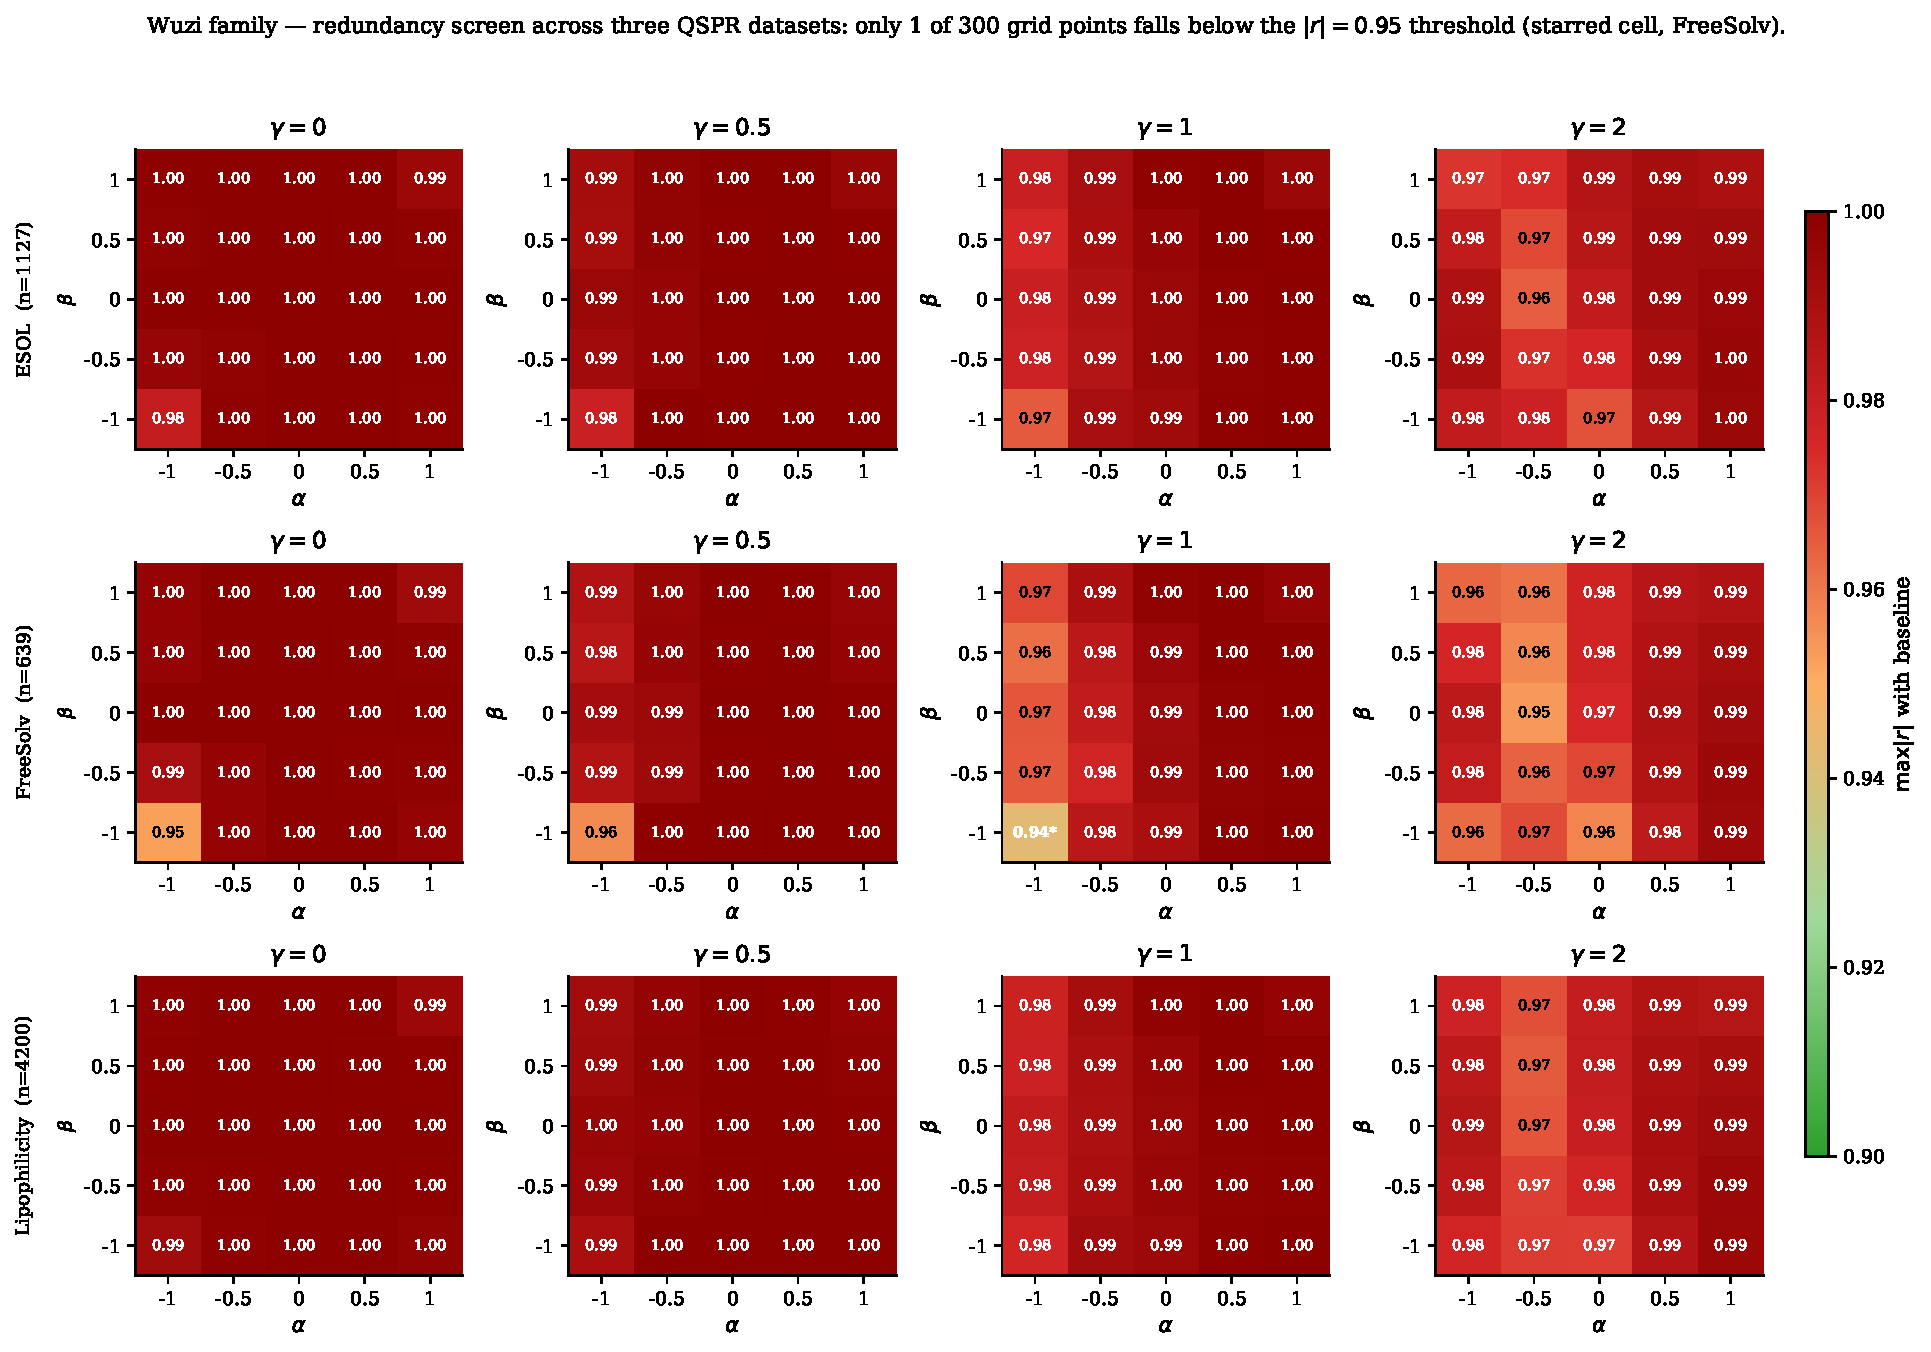
\includegraphics[width=\linewidth]{fig5b_wuzi_param_heatmaps_all.pdf}
\caption{$\max|r|$ between the Wuzi index at each $(\alpha,\beta,\gamma)$
grid point and any of the $30$ classical baseline indices, across
the three datasets (rows) and four $\gamma$ slices (columns).
The starred cell (FreeSolv, $(-1,-1,1)$) is the only grid point
that falls below $|r|=0.95$; at the same parameter triple the
partial correlation with the target is identically zero on all three
datasets.}
\label{fig:wuzi_grid_all}
\end{figure}

\subsubsection{Consistency with the BID-basis observation}

Corollary~\ref{cor:bid_redundancy} predicts that no parametric BID
family can have effective dimension above $10$ on $\mathcal{G}_4$.
With three principal components capturing $95\%$ of the baseline
variance, the empirical effective rank is much lower than $10$; a
new BID index has at most a $7$-dimensional ``budget''
within which to be statistically independent of the leading PCA
factors. The empirical screening verdict that no Wuzi parameter
point clears $|r|<0.95$ \emph{and} provides meaningful partial
correlation is consistent with this structural constraint.

\subsubsection{Threshold sensitivity of the Wuzi verdict}\label{sub:threshold_sensitivity}

A standard concern with any thresholded screen is whether the
qualitative verdict survives reasonable variation in the cutoffs
$(\tau_r, \tau_{\mathrm{pcor}})$. Table~\ref{tab:threshold_sensitivity}
tabulates the Wuzi $100$-point grid pairwise-pass counts at
$\tau_r \in \{0.90, 0.95, 0.99\}$ and the combined-diagnostic-pass
counts across the full $3 \times 3$ grid of
$\tau_r \in \{0.90, 0.95, 0.99\}$ and
$\tau_{\mathrm{pcor}} \in \{0.05, 0.10, 0.20\}$
on each of the three QSPR datasets (full table in
\texttt{results/paper2\_threshold\_sensitivity.csv}).

\begin{table}[h]
\centering
\small
\caption{Wuzi $100$-point grid: pass counts under threshold variation. Top block: pairwise screen only ($\max_b\lvert r(W, X_b)\rvert < \tau_r$). Bottom block: combined diagnostic (pairwise pass \emph{and} $\lvert\mathrm{pcor}(W, y \mid X)\rvert \ge \tau_{\mathrm{pcor}}$) across the full $3 \times 3$ threshold grid.}
\label{tab:threshold_sensitivity}
\begin{tabular}{lccc}
\toprule
& \multicolumn{3}{c}{Pairwise pass count ($\tau_r$)}\\
\cmidrule(lr){2-4}
Dataset & $\tau_r = 0.90$ & $\tau_r = 0.95$ & $\tau_r = 0.99$\\
\midrule
ESOL          & $0$ & $0$ & $27$\\
FreeSolv      & $0$ & $1$ & $37$\\
Lipophilicity & $0$ & $0$ & $30$\\
\bottomrule
\end{tabular}

\vspace{0.6em}

\begin{tabular}{l|ccc|ccc|ccc}
\toprule
& \multicolumn{3}{c|}{$\tau_r = 0.90$} & \multicolumn{3}{c|}{$\tau_r = 0.95$} & \multicolumn{3}{c}{$\tau_r = 0.99$}\\
$\tau_{\mathrm{pcor}}$ & $.05$ & $.10$ & $.20$ & $.05$ & $.10$ & $.20$ & $.05$ & $.10$ & $.20$\\
\midrule
ESOL          & $0$ & $0$ & $0$ & $0$ & $0$ & $0$ & $0$ & $0$ & $0$\\
FreeSolv      & $0$ & $0$ & $0$ & $0$ & $0$ & $0$ & $0$ & $0$ & $0$\\
Lipophilicity & $0$ & $0$ & $0$ & $0$ & $0$ & $0$ & $0$ & $0$ & $0$\\
\bottomrule
\end{tabular}

\vspace{0.3em}
\noindent\small{Combined-diagnostic pass count of the Wuzi $100$-point grid across the full $\{0.90, 0.95, 0.99\} \times \{0.05, 0.10, 0.20\}$ threshold grid (nine $(\tau_r, \tau_{\mathrm{pcor}})$ combinations).}
\end{table}

\noindent The qualitative conclusion is stable across the tested
thresholds: \emph{no} Wuzi grid point clears the combined
diagnostic at any of the nine $(\tau_r, \tau_{\mathrm{pcor}})$
combinations in $\{0.90, 0.95, 0.99\} \times \{0.05, 0.10, 0.20\}$
on any of the three datasets. Relaxing the pairwise threshold to
$\tau_r = 0.99$ admits roughly a third of grid points through the
pairwise screen ($27$, $37$, $30$ of $100$), but none of those
survive even the loosest partial-correlation cutoff
$\tau_{\mathrm{pcor}} = 0.05$. The exact pass counts are
threshold-dependent; the conclusion that the Wuzi family lacks
independent linear QSPR signal on these datasets under the
$30$-index baseline is not.

\subsection{Case study 2: alternative-family candidates across four datasets}\label{sec:novel_case}

\noindent\emph{Scope note.} This case study screens twenty
alternative-family candidate indices on all four benchmarks
(ESOL, FreeSolv, Lipophilicity, BBBP), so the headline pattern
``$15$--$17/20$ clear the pairwise screen but only $0$--$4/20$
also clear the partial-correlation screen'' is a cross-dataset
finding, not a single-dataset case study. The candidates are
identical across datasets; the per-dataset verdict differs because
the residual signal under the $30$-index baseline differs by
target. We make no claim that any individual passer is a useful
descriptor; the screening verdict is a redundancy diagnostic, not
a chemical-utility certification. The candidates were chosen as
five distinct design philosophies (information-theoretic,
centrality, motif, eccentricity, spectral-hybrid) to test that
the screening conclusion generalises beyond the BID-family case
study of \S\ref{sec:wuzi_case}.

We screen $20$ candidate indices on the four datasets, drawn from
the five alternative design families described below.

\begin{table}[h]
\centering
\caption{Twenty candidate indices grouped by design family.}
\label{tab:candidates}
\begin{tabular}{ll}
\toprule
Family & Candidate indices (working names)\\
\midrule
Information-theoretic (5) & InfoH\_deg, InfoH\_dist, InfoH\_spec, InfoH\_ecc, Bonchev\_Id\\
Centrality (5) & Btw\_sum, Cls\_sum, Eig\_sum, Harm\_cent, Btw\_var\\
Motif (4) & Triangles, MeanClust, FourCyc, CutVerts\\
Eccentricity (3) & TotEcc, Radius, MeanEcc\\
Spectral-hybrid (3) & AlgConn, Rho$\times$Dia, EE$\times$W\\
\bottomrule
\end{tabular}
\end{table}

\noindent\emph{Disclaimer.} None of the $20$ candidates is claimed
to be newly invented. Each has prior chemistry literature (the
information-theoretic group draws on Cao--Dehmer--Shi and related
entropy-style proposals; the centrality group on textbook graph
centrality measures; the motif and eccentricity groups on
standard graph invariants; the spectral-hybrid group on
combinations of standard spectral quantities). They appear here
purely as screening targets to test whether candidates from
different design philosophies escape the redundancy ceiling on
ESOL; the full per-candidate citation list is collected in
\texttt{docs/literature\_notes.md} in the companion repository.

\subsubsection{Screening verdict across the four datasets}

Table~\ref{tab:novel_combined} reports the per-dataset pairwise and
combined pass counts. The pairwise $|r|<0.95$ screen alone admits
$15$--$17$ of the $20$ candidates on every dataset; the combined
diagnostic that additionally requires
$|\mathrm{pcor}|\ge 0.10$ admits only $0$--$4$. The pattern is
consistent: the pairwise screen is uniformly over-permissive, and
the combined diagnostic is sharper on FreeSolv ($1/20$ pass),
BBBP ($2/20$), and Lipophilicity ($0/20$) than on ESOL ($4/20$).

For BBBP (binary target) the partial-correlation diagnostic is
computed via the linear probability model: we fit
$y \sim X_{\mathrm{baseline}}$ as ordinary least squares against
the $0/1$ class indicator and take residuals; the candidate is
then residualised by the same baseline and Pearson-correlated
with the residual class indicator. This is the standard
LPM-based partial correlation; it puts the BBBP row of
Table~\ref{tab:novel_combined} on the same scale as the three
regression rows. A logistic-pseudo-$R^2$ alternative
(Tjur's coefficient) is recorded as future work in
\S\ref{sub:limitations}.

\begin{table}[h]
\centering
\caption{Combined screening verdict on the $20$ candidates against the $30$-index baseline on each of the four MoleculeNet benchmarks. $\mathrm{PASS}_{\mathrm{pair}}$ = max $|r| < 0.95$; $\mathrm{PASS}_{\mathrm{combined}}$ = max $|r| < 0.95$ AND $|\mathrm{pcor}|\ge 0.10$. Per-dataset combined passers are listed in the footnote.}
\label{tab:novel_combined}
\begin{tabular}{lcccr}
\toprule
Dataset & $n$ & $\mathrm{PASS}_{\mathrm{pair}}$ / $20$ & $\mathrm{PASS}_{\mathrm{combined}}$ / $20$ & $\max|\mathrm{pcor}|$\\
\midrule
ESOL          & $1\,127$ & $15$ & $4$ & $0.154$\\
FreeSolv      & $\phantom{0}639$  & $15$ & $1$ & $0.129$\\
Lipophilicity & $4\,200$ & $16$ & $0$ & $0.077$\\
BBBP$^\ddag$  & $2\,039$ & $17$ & $2$ & $0.225$\\
\bottomrule
\end{tabular}

\vspace{0.4em}
\noindent\small{Combined passers per dataset:
ESOL: $\mathrm{InfoH\_deg}\,(0.154)$, CutVerts $(0.118)$, FourCyc $(0.112)$, MeanEcc $(0.109)$.
FreeSolv: Triangles $(0.107)$.
Lipophilicity: none.
BBBP: $\mathrm{InfoH\_deg}\,(0.225)$, $\mathrm{InfoH\_dist}\,(\approx 0.16)$.
$^\ddag$ BBBP partial correlation computed via LPM (see text).}
\end{table}

The headline pattern: the pairwise $|r|<0.95$ screen alone is
over-permissive on every dataset --- $75$--$85\%$ of candidates
clear it --- but the combined diagnostic that additionally
requires $|\mathrm{pcor}|\ge 0.10$ leaves $0$--$4$ candidates as
plausible carriers of independent linear signal under the
$30$-index baseline. The strongest passer across the four
datasets is $\mathrm{InfoH\_deg}$ on BBBP at $|\mathrm{pcor}|=0.225$;
no other candidate reaches $|\mathrm{pcor}|>0.2$ on any dataset.
Detailed per-candidate numbers are in
\texttt{results/novel\_candidates\_experiment/novel\_candidates\_multidataset.csv}.

These per-dataset combined passers should be read as
``residual-signal positive on that specific target under the
$30$-index linear baseline'', not as useful QSPR descriptors;
the diagnostic is a redundancy filter, not a utility
certification.

\subsubsection{Structural interpretation of the four ESOL passers}\label{sec:passer_analysis}

We focus the structural reading on ESOL because the four ESOL
passers span the widest set of design philosophies among the four
datasets and so best illustrate \emph{why} the partial-correlation
diagnostic catches signal that pairwise correlation misses. The
qualitative argument transfers to the FreeSolv (Triangles) and BBBP
($\mathrm{InfoH\_deg}$, $\mathrm{InfoH\_dist}$) passers; the
specific structural reading below is ESOL-only.

The four candidates that clear the combined diagnostic on ESOL span
three distinct design philosophies, and each computes a graph
property that is \emph{not} expressible as a sum of per-edge
contributions:

\begin{itemize}
\item $\mathrm{InfoH\_deg}$, the Shannon entropy of the degree
multiplicities of $G$, is a logarithmic functional of the degree
\emph{distribution}, not of the degree sequence summed edgewise.
\item $\mathrm{CutVerts}$, the number of articulation points of $G$,
is a vertex-connectivity invariant: the count of vertices whose
removal disconnects $G$. It depends on the global block structure
of $G$, not on local edge properties.
\item $\mathrm{FourCyc}$, the number of induced $4$-cycles, captures
a cycle-counting property of $G$. On hydrogen-suppressed molecular
graphs of order $n \le 30$ it is small (often zero) and captures
ring-substructure information disjoint from degree-based measures.
\item $\mathrm{MeanEcc}$, the mean of the vertex eccentricities, is
a distance-based scalar that depends on shortest-path lengths
rather than on degrees.
\end{itemize}

This shared structural feature explains why all four can clear the
partial-correlation threshold even when their pairwise correlation
against an individual baseline is high. $\mathrm{MeanEcc}$, for
example, has $\max |r| = 0.930$ against the modified second
Zagreb index $mM_2$ on ESOL --- well above any natural redundancy
threshold for a pair of degree-based indices --- but it still
retains $|\mathrm{pcor}| = 0.109$ once the full $30$-index linear
span is regressed out. Pairwise correlation against a single
baseline does not preclude residual signal orthogonal to the
$30$-dimensional baseline subspace, and the partial-correlation
diagnostic is the component of the combined diagnostic that catches
this. By contrast, the $11$ candidates that clear the pairwise
screen with $|\mathrm{pcor}| < 0.10$ are well-approximated by a
linear combination of the $30$ baseline indices: high pairwise
$|r|$ against \emph{one} baseline is neither necessary nor
sufficient for redundancy against the \emph{full} baseline.

We emphasise that the four passing partial correlations are small
in absolute terms ($0.109 \le |\mathrm{pcor}| \le 0.154$, all under
$0.2$). The reading we recommend is the structural one --- the
passers occupy a subspace of feature space outside the linear span
of the $30$-index baseline --- not a chemical-utility one. Whether
any of $\mathrm{InfoH\_deg}$, $\mathrm{CutVerts}$, $\mathrm{FourCyc}$,
or $\mathrm{MeanEcc}$ actually improves QSPR performance on $\log S$
or any other endpoint is a separate question, answered in part by
the ML benchmark of Section~\ref{sec:ml_benchmark} and ultimately
requiring downstream validation on tasks beyond ESOL.

\subsection{Downstream ML benchmark: does screening preserve predictive performance?}\label{sec:ml_benchmark}

The case studies of Sections~\ref{sec:wuzi_case} and~\ref{sec:novel_case}
demonstrate that the combined diagnostic is more selective than the
pairwise screen alone. They do not yet demonstrate that the criterion
is useful for building predictive QSPR models. This section closes
that gap: we train a RandomForest (300 trees, fixed seed,
\texttt{class\_weight="balanced"} for classification) on each of four
datasets under four feature configurations across $5$-fold
cross-validation, and report whether the screened feature set
matches the full-baseline model's predictive performance within
CV noise.

\textbf{Datasets.} The three QSPR regression benchmarks of
Section~\ref{sec:datasets} are augmented with a fourth dataset to
test that the pipeline generalizes beyond regression:
\textbf{BBBP} (\cite{Martins2012BBBP} via~\cite{MoleculeNet}), $2\,050$
molecules in the source CSV of which $2\,039$ parse via RDKit and
enter the screen; binary target ``blood-brain barrier
penetration''; class distribution approximately $3{:}1$
(positive:negative), handled with a class-balanced RandomForest.

\textbf{Configurations and cross-validation protocol.} $5$-fold
cross-validation, stratified for the classification task, identical
folds across all configurations so the comparison isolates the
effect of feature selection. All feature selection is performed
\emph{inside each training fold} to avoid test-fold information
leakage.
\begin{itemize}
\item \textbf{full}: all $30$ baseline indices.
\item \textbf{pca\_95}: top-$k$ principal components of the
training-fold-standardized baseline at $95\%$ cumulative variance
($k=3$ on all four datasets, every fold).
\item \textbf{pairwise\_pruned}: greedy redundancy filter at
$|r| < 0.95$ on the training fold (keep one representative per
correlation cluster).
\item \textbf{combined\_pruned}: pairwise filter plus
$|\mathrm{pcor}(z, y \mid X_{\mathrm{others}})| \ge 0.10$ on the
training fold's pairwise-pruned set.
\end{itemize}

\textbf{Results.} Table~\ref{tab:ml_benchmark} and
Figure~\ref{fig:ml_benchmark} summarize the per-dataset, per-configuration
RandomForest performance (mean $\pm$ std across the $5$ folds) and
mean feature count.

\begin{table}[h]
\centering
\small
\caption{RandomForest $5$-fold cross-validation performance under four feature configurations. Regression metric is RMSE (lower is better); classification metric is ROC-AUC (higher is better). Reported as mean $\pm$ std across folds. The \texttt{combined\_pruned} screen retained zero features in $4$ of $5$ folds on Lipophilicity (the RMSE shown is from the single fold that retained one feature).}
\label{tab:ml_benchmark}
\begin{tabular}{lccccrr}
\toprule
Dataset & \texttt{full} & \texttt{pca\_95} & \texttt{pairwise\_pruned} & \texttt{combined\_pruned} & full $n$ & pairwise $n$\\
\midrule
ESOL          & $1.437 \pm 0.102$ & $1.455 \pm 0.096$ & $1.435 \pm 0.087$ & $1.475 \pm 0.123$ & $30$ & $7.4$ ($7$--$9$)\\
FreeSolv      & $3.537 \pm 0.228$ & $3.544 \pm 0.264$ & $3.540 \pm 0.224$ & $3.561 \pm 0.300$ & $30$ & $8.0$\\
Lipophilicity & $1.030 \pm 0.024$ & $1.065 \pm 0.018$ & $1.028 \pm 0.022$ & $1.287$ ($1/5$ folds) & $30$ & $8.0$\\
BBBP          & $0.846 \pm 0.006$ & $0.818 \pm 0.014$ & $0.860 \pm 0.010$ & $0.840 \pm 0.010$ & $30$ & $6.0$\\
\bottomrule
\end{tabular}
\end{table}

\begin{figure}[h]
\centering
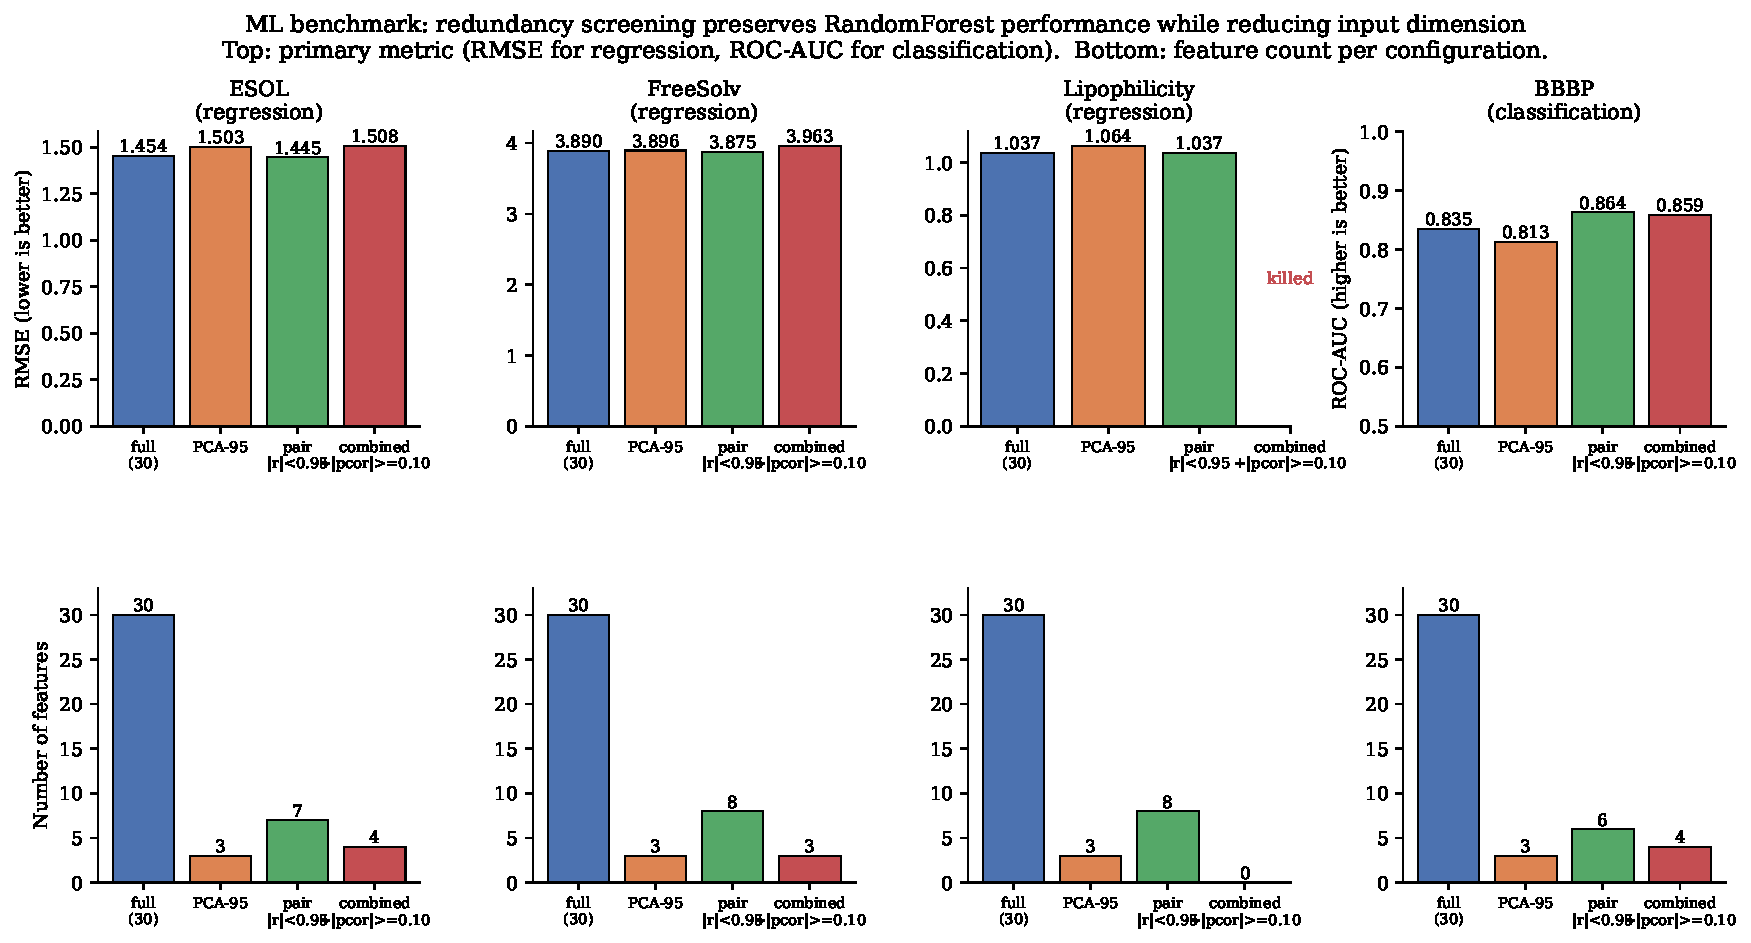
\includegraphics[width=\linewidth]{fig9_ml_benchmark.pdf}
\caption{Downstream ML benchmark on four datasets, $5$-fold cross
validation. Top row: primary metric (RMSE for the three regression
panels, ROC-AUC for BBBP), mean $\pm$ std across folds. Bottom row:
mean feature count per configuration, error bar = min--max range
across folds. The pairwise screen matches the full-baseline
RandomForest on every dataset, with mean differences below CV
noise, while using roughly $4\times$ (range $3.75$--$5\times$)
fewer features. On Lipophilicity the strict combined screen retains
zero features in $4$ of $5$ folds.}
\label{fig:ml_benchmark}
\end{figure}

\textbf{Interpretation.} On the four MoleculeNet benchmarks tested,
the \texttt{pairwise\_pruned} configuration matches \texttt{full}
within CV noise: mean RMSE differences are $|\Delta| \le 0.005$ on
all three regression datasets and the mean and std intervals
overlap. On BBBP, \texttt{pairwise\_pruned} attains ROC-AUC
$0.860 \pm 0.010$ versus \texttt{full} at $0.846 \pm 0.006$; the
mean delta is $0.014$, with marginal overlap of the std bands.
This is best read as ``matches or marginally exceeds within CV
noise'' rather than a definitive improvement. The PCA-95
configuration consistently underperforms by $\approx 0.02$ RMSE or
$\approx 0.03$ ROC-AUC, suggesting that the principal directions
of the standardized $30$-index baseline are not the
target-relevant directions for these specific QSPR problems.

The stricter \texttt{combined\_pruned} configuration is more
aggressive and on the regression datasets shows a small performance
penalty (mean RMSE up to $0.04$ higher than \texttt{full}, still
overlapping std bands). On Lipophilicity the combined screen
retains zero features in $4$ of the $5$ folds, an honest failure
mode that reflects the dataset's weak topology-to-$\log D$
partial-correlation structure (no pairwise-pruned index has
$|\mathrm{pcor}| \ge 0.10$ with $\log D$ on most folds). The
threshold $|\mathrm{pcor}| = 0.10$ should be relaxed (or replaced
with a target-correlation rank cut) on datasets where the underlying
topology-target relationship is weak. We do not recommend the
combined screen as a hard filter; it is best read as a diagnostic
that flags ``low pairwise correlation but low partial correlation
too'' --- which is exactly the failure mode the Wuzi family at
$(-1,-1,1)$ exhibits.

\subsubsection{Comparison to LASSO, ElasticNet, mRMR, Boruta, and L1-logistic feature selection}\label{sub:lasso_comparator}

To position the pairwise / combined diagnostic against a broader
set of feature-selection comparators, we evaluate five external
methods alongside the pipeline configurations of
Table~\ref{tab:ml_benchmark}:
\begin{itemize}
\item LASSO with $5$-fold CV-tuned $\alpha$ (three regression datasets);
\item ElasticNet with CV-tuned $\alpha$ and $\ell_1$-ratio
$\in \{0.3, 0.5, 0.7, 0.9\}$ (three regression datasets);
\item mRMR top-$k$ with $k$ matched to the pairwise-pruned mean
feature count of Table~\ref{tab:ml_benchmark} (all four datasets);
\item Boruta with RandomForest base estimator (all four datasets);
\item $\ell_1$-Logistic with CV-tuned $C$ (BBBP only; the
classification analog of LASSO).
\end{itemize}
The cached $30$-index baseline matrix and the same $5$-fold splits
as Table~\ref{tab:ml_benchmark} are used; for mRMR and Boruta we
evaluate the selected subset under ordinary linear regression
(regression) or logistic regression (BBBP) to keep the comparator
linear-model class consistent with LASSO. The screen-pipeline rows
remain RandomForest, so the comparison is intentionally across two
model classes; we read it as a sanity check that the pairwise screen
is not being compared to a strawman, not as a head-to-head model
benchmark.

\begin{table}[h]
\centering
\small
\caption{Screen-pipeline configurations (RandomForest, rows from Table~\ref{tab:ml_benchmark}) vs.\ five external feature-selection comparators (LASSO, ElasticNet, mRMR, Boruta, $\ell_1$-Logistic) on the four MoleculeNet benchmarks. Regression metric is RMSE (lower is better); classification metric for BBBP is ROC-AUC (higher is better). Reported as mean across 5 folds with the same seed; standard deviations in \texttt{results/paper2\_feature\_selection\_comparison.csv}.}
\label{tab:fs_comparison}
\begin{tabular}{llrr}
\toprule
Dataset & Configuration & Metric & Mean $n$ features\\
\midrule
ESOL & \texttt{full} (RF)                 & RMSE $1.437$ & $30.0$\\
     & \texttt{pairwise\_pruned} (RF)     & RMSE $1.435$ & $\phantom{0}7.4$\\
     & \texttt{combined\_pruned} (RF)     & RMSE $1.475$ & $\phantom{0}4.4$\\
     & LASSO (linear, CV)                 & RMSE $1.545$ & $14.6$\\
     & ElasticNet (linear, CV)            & RMSE $1.546$ & $16.2$\\
     & mRMR $k{=}7$ (linear)              & RMSE $1.654$ & $\phantom{0}7.0$\\
     & Boruta + RF (linear scoring)       & RMSE $1.620$ & $10.0$\\
\midrule
FreeSolv & \texttt{full} (RF)             & RMSE $3.537$ & $30.0$\\
         & \texttt{pairwise\_pruned} (RF) & RMSE $3.540$ & $\phantom{0}8.0$\\
         & \texttt{combined\_pruned} (RF) & RMSE $3.561$ & $\phantom{0}3.2$\\
         & LASSO (linear, CV)             & RMSE $3.527$ & $13.4$\\
         & ElasticNet (linear, CV)        & RMSE $3.515$ & $18.6$\\
         & mRMR $k{=}8$ (linear)          & RMSE $3.618$ & $\phantom{0}8.0$\\
         & Boruta + RF (linear scoring)   & RMSE $3.588$ & $\phantom{0}2.0$\\
\midrule
Lipophilicity & \texttt{full} (RF)        & RMSE $1.030$ & $30.0$\\
              & \texttt{pairwise\_pruned} (RF) & RMSE $1.028$ & $\phantom{0}8.0$\\
              & \texttt{combined\_pruned} (RF) & RMSE $1.287^{\,\dagger}$ & $\phantom{0}0.2$\\
              & LASSO (linear, CV)        & RMSE $1.130$ & $15.6$\\
              & ElasticNet (linear, CV)   & RMSE $1.130$ & $17.8$\\
              & mRMR $k{=}8$ (linear)     & RMSE $1.142$ & $\phantom{0}8.0$\\
              & Boruta + RF (linear scoring) & RMSE $1.144$ & $\phantom{0}5.0$\\
\midrule
BBBP & \texttt{full} (RF)                 & AUC $0.846$ & $30.0$\\
     & \texttt{pairwise\_pruned} (RF)     & AUC $0.860$ & $\phantom{0}6.0$\\
     & \texttt{combined\_pruned} (RF)     & AUC $0.840$ & $\phantom{0}4.0$\\
     & $\ell_1$-Logistic (CV)             & AUC $0.790$ & $13.6$\\
     & mRMR $k{=}6$ (logistic)            & AUC $0.747$ & $\phantom{0}6.0$\\
     & Boruta + RF (logistic scoring)     & AUC $0.791$ & $23.0$\\
\bottomrule
\end{tabular}

\vspace{0.5em}
\noindent\small{$^\dagger$ Strict combined screen degenerates: retains zero features in $4/5$ folds; the RMSE shown is from the single fold that retained one feature. See \S\ref{sub:limitations}.}
\end{table}

The headline reading: on \emph{all four datasets}, the
\texttt{pairwise\_pruned} RandomForest matches or beats every
external feature-selection comparator we tested, with feature
counts in the range $6$--$8$ versus $6$--$23$ for the comparators.
On ESOL, \texttt{pairwise\_pruned} RMSE $1.435$ at $7.4$ features
beats LASSO ($1.545$ at $14.6$ features) by $0.11$ RMSE and beats
mRMR-$k{=}7$ by $0.22$ RMSE. On BBBP, \texttt{pairwise\_pruned}
ROC-AUC $0.860$ at $6$ features beats $\ell_1$-Logistic by
$0.07$ AUC and beats mRMR-$k{=}6$ by $0.11$ AUC. We caveat that
this comparison crosses two model classes (RandomForest for the
screen-pipeline rows, linear for the comparators), so the
mechanical reading is ``pairwise-pruned RandomForest is at least
competitive with linear-model LASSO / ElasticNet / mRMR / Boruta /
$\ell_1$-Logistic at matched feature count'' rather than a
head-to-head model-architecture benchmark. Full per-fold standard
deviations are in
\texttt{results/paper2\_feature\_selection\_comparison.csv}.

% =====================================================================
\section{Discussion}\label{sec:discussion}
% =====================================================================

The two case studies and the cross-validated ML benchmark together
support a single methodological reading. Section~\ref{sec:wuzi_case}
shows that the pairwise diagnostic alone admits a parameter setting
(the Wuzi FreeSolv point at $(-1, -1, 1)$) that clears
$|r| < 0.95$ yet has multi-dimensional partial correlation
identically zero against the baseline on every dataset --- the
failure mode the combined diagnostic of Table~\ref{tab:decision} is
designed to catch. Section~\ref{sec:ml_benchmark} shows that the
combined screen is best read as a diagnostic rather than as a hard
filter: it flags the Wuzi failure mode but degenerates on
Lipophilicity, where the topology-to-$\log D$ partial-correlation
structure is too weak for any pairwise-pruned index to clear
$|\mathrm{pcor}| \ge 0.10$. The threshold should therefore be tied
to the QSPR utility loss the analyst is willing to tolerate, not
treated as a fixed cutoff.

Theorem~\ref{thm:bid} (Edge-Degree-Pair Basis) gives the structural
reason for the empirical redundancy ceiling observed across the
three datasets: the dimension-$10$ cap is intrinsic to the BID
construction on $\mathcal{G}_4$ rather than an artefact of any
particular dataset.

% =====================================================================
\section{Limitations and open questions}\label{sec:limitations}
% =====================================================================

We catalogue the assumptions and the open questions explicitly so
that downstream users of the pipeline can read off where its
guarantees stop and where additional methodological work is needed.

\subsection{Limitations of the present pipeline}\label{sub:limitations}

We catalogue the formal limitations as a reviewer-facing list so
the scope of every claim is bounded explicitly:

\begin{enumerate}
\item \textbf{Linear diagnostics only.} The pipeline is built on
Pearson correlation, OLS partial correlation, and PCA. Non-linear
relationships between a candidate index and the target, or between
the candidate and the baseline, are not captured. Distance
correlation, rank-based equivalents (Spearman), or
mutual-information-style estimators would close the non-linearity
gap at the cost of looser interpretability.

\item \textbf{Threshold convention.} $\tau_r = 0.95$ for the
pairwise screen and $\tau_{\mathrm{pcor}} = 0.10$ for the
partial-correlation condition are conventional but arbitrary
cutoffs and should be tuned to the QSPR-utility loss the analyst
is willing to tolerate. The qualitative conclusions of
\S\ref{sub:threshold_sensitivity} (no Wuzi grid point passes the
combined diagnostic on any dataset, at any of the nine tested
$(\tau_r, \tau_{\mathrm{pcor}})$ combinations) are stable; the
\emph{exact} pass counts are not.

\item \textbf{Alternative-family pass-counts are
single-target, not chemical-utility claims.} The $20$-candidate
experiment of \S\ref{sec:novel_case} is replicated across all four
datasets, and the qualitative conclusion (pairwise admits $15$--$17$
of $20$ candidates; combined admits $0$--$4$) is consistent across
ESOL, FreeSolv, Lipophilicity, and BBBP. However, the individual
combined passers (e.g.\ $\mathrm{InfoH\_deg}$ on ESOL and BBBP,
Triangles on FreeSolv) should still be interpreted as
``residual-signal positive on that specific target under the
$30$-index linear baseline'', not as useful QSPR descriptors in
absolute terms.

\item \textbf{Combined diagnostic should not be used as a hard
filter.} On Lipophilicity the strict combined screen
($\tau_{\mathrm{pcor}} \ge 0.10$) retains zero features in $4/5$
ML-benchmark folds; the pairwise screen alone reduces feature count
by ${\sim}4\times$ while preserving predictive performance within
CV noise, but the partial-correlation diagnostic should be read as
evidence about residual target signal rather than as an automatic
feature-selection rule. The Wuzi Lipophilicity result of
Table~\ref{tab:wuzi_verdict_paper1} and the Lipo ML-benchmark
column of Table~\ref{tab:ml_benchmark} both illustrate this
failure mode honestly.

\item \textbf{RandomForest is one model class; the
linear-comparator benchmark crosses model classes.}
Section~\ref{sub:lasso_comparator} compares the screen-pipeline
configurations against LASSO, ElasticNet, mRMR, Boruta, and
$\ell_1$-Logistic on all four datasets. The screen-pipeline rows
use a RandomForest, and the comparators use linear regression
(regression datasets) or logistic regression (BBBP); the
\texttt{pairwise\_pruned} RandomForest matches or beats every
comparator at matched feature count. The reported comparison is
therefore best read as ``pairwise-pruned RandomForest is at least
competitive with linear-model LASSO / ElasticNet / mRMR / Boruta /
$\ell_1$-Logistic'' rather than as a head-to-head
model-architecture benchmark; a fully matched comparison
(linear-model screen-pipeline rows or tree-ensemble comparators
such as XGBoost-mRMR) is left as future work.

\item \textbf{BID dimension bound covers $\Delta \le 4$ only.} The
Edge-Degree-Pair Basis bound (Theorem~\ref{thm:bid}) is sharp on
$\mathcal{G}_4$, which covers C / N / O / halogen and most S
chemistry; organometallics, hypervalent species, and inorganic
chemistry fall outside the dimensional cap and require a separate
analysis. Likewise, non-BID parametric families (distance-based,
spectral, mixed) are not bounded by Theorem~\ref{thm:bid} and a
structural dimension bound analogous to it for these families is
open.

\item \textbf{Single-scalar indices only.} The pipeline screens one
scalar at a time; a vector descriptor, or a small set of jointly
designed scalars, may be redundant individually but informative
collectively.
\end{enumerate}

\subsection{Open methodological questions}

The following directions are natural extensions of the framework.
We list them as open questions rather than completed work; a
formal study of any one of them would be a follow-up project.

\begin{enumerate}
\item \textbf{Extension beyond the BID family.} A structural
dimension bound analogous to Theorem~\ref{thm:bid} for
distance-based, spectral, or mixed-family parametric topological
indices is open.
\item \textbf{Threshold sensitivity.} A formal change-point
analysis of the pipeline conclusions as a function of the
thresholds $(\tau, \tau_{\mathrm{pcor}})$ would replace the
conventional cutoffs with data-driven equivalents.
\item \textbf{Non-linear diagnostics.} Distance correlation and
mutual-information-style estimators offer non-linear redundancy
measures that complement the linear Pearson / OLS / PCA core. A
joint diagnostic combining linear and non-linear redundancy
checks has not been validated against a QSPR benchmark.
\item \textbf{Web deployment.} A web-deployed version of the
pipeline that accepts a SMILES file and a candidate-index Python
function and returns the four diagnostics in seconds would lower
the activation energy for routine use.
\item \textbf{Two-stage pipeline-then-feature-selection vs.
end-to-end feature-selection on full QSPR endpoints.}
Section~\ref{sub:lasso_comparator} reports per-dataset
configuration-level scores under a fixed RandomForest backbone;
a head-to-head benchmark of \emph{pipeline-then-feature-selection}
(use the combined diagnostic to drop redundant candidates, then
LASSO / mRMR / Boruta the survivors) versus \emph{end-to-end
feature-selection-only} (LASSO / mRMR / Boruta on the
$30$-index baseline directly) on a full downstream QSPR endpoint
is open. Sequential composition is expected to be at least as
strong as either component alone, but this has not been
empirically verified here.
\end{enumerate}

% =====================================================================
\section{Conclusion}
% =====================================================================

We have introduced an open-source orthogonality-screening pipeline
for scalar topological indices, applied it across three
MoleculeNet QSPR regression benchmarks and one classification
benchmark, and validated that the pairwise screen preserves
predictive performance within CV noise at roughly $4\times$ fewer
features. The Edge-Degree-Pair Basis (Theorem~\ref{thm:bid})
gives the structural reason that the empirical redundancy
ceiling observed across the three datasets is intrinsic to the
bond-incident-degree construction on $\mathcal{G}_4$ rather than
an artefact of any particular dataset. The combined diagnostic of
low maximum pairwise correlation against a classical baseline
\emph{and} non-negligible partial correlation with the QSPR target
operationalises the ``does a new index carry independent
information'' question as a pre-flight check for proposed new
indices; open methodological questions (non-linear diagnostics,
non-BID extensions of Theorem~\ref{thm:bid}, threshold
sensitivity, web deployment) are catalogued in
Section~\ref{sec:limitations}.

% =====================================================================
\section*{Data and code availability}
% =====================================================================

Code, datasets, and figures are publicly available at
\url{https://github.com/Singati2/topological-index-orthogonality}.
The pipeline runs in seconds per benchmark on a single laptop;
adding a candidate index requires a short Python function on the
hydrogen-suppressed molecular graph.

% =====================================================================
\section*{Acknowledgements}
% =====================================================================

The authors thank colleagues for discussions of the screening
protocol and the alternative-family candidate index set. Funding
sources and institutional support to be acknowledged in the final
version of the manuscript.

% =====================================================================
\begin{thebibliography}{99}
% =====================================================================
\small

\bibitem{Wiener1947}
H.~Wiener,
\emph{Structural determination of paraffin boiling points},
J.~Am.~Chem.~Soc.~\textbf{69} (1947), 17--20.

\bibitem{Randic1975}
M.~Randi\'c,
\emph{On characterization of molecular branching},
J.~Am.~Chem.~Soc.~\textbf{97} (1975), 6609--6615.

\bibitem{Gutman1972}
I.~Gutman and N.~Trinajsti\'c,
\emph{Graph theory and molecular orbitals},
Chem.~Phys.~Lett.~\textbf{17} (1972), 535--538.

\bibitem{MovahediGutmanRedzepovicFurtula2026}
F.~Movahedi, I.~Gutman, I.~Red\v{z}epovi\'c, and B.~Furtula,
\emph{Diminished Sombor index of graphs},
MATCH Commun.~Math.~Comput.~Chem.~\textbf{95} (2026), 141--162.

\bibitem{BorovicaninDasFurtulaGutman2017Zagreb}
B.~Borovi\'canin, K.~C.~Das, B.~Furtula, and I.~Gutman,
\emph{Bounds for Zagreb indices},
MATCH Commun.~Math.~Comput.~Chem.~\textbf{78} (2017), 17--100.
(Reprinted as a chapter in I.~Gutman, B.~Furtula, K.~C.~Das,
E.~Milovanovi\'c, and I.~Milovanovi\'c (eds.),
\emph{Bounds in Chemical Graph Theory --- Mainstreams},
Mathematical Chemistry Monographs MCM-20,
University of Kragujevac, 2017, pp.~67--153.)

\bibitem{Albertson1997}
M.~O.~Albertson,
\emph{The irregularity of a graph},
Ars Combin.~\textbf{46} (1997), 219--225.

\bibitem{VukicevicFurtula2009GA}
D.~Vuki\v{c}evi\'c and B.~Furtula,
\emph{Topological index based on the ratios of geometrical
and arithmetical means of end-vertex degrees of edges},
J.~Math.~Chem.~\textbf{46}(4) (2009), 1369--1376.
\url{https://doi.org/10.1007/s10910-009-9520-x}.

\bibitem{Paper1_Wuzi}
A.~Natarajan, G.~Shiwakoti, M.~Arockiaraj,
\emph{The Wuzi Index Family and the Ten-Dimensional Ceiling of Molecular BID Descriptors},
in preparation, 2026.
(Companion mathematical paper.)

\bibitem{MoleculeNet}
Z.~Wu, B.~Ramsundar, E.~N.~Feinberg, J.~Gomes, C.~Geniesse,
A.~S.~Pappu, K.~Leswing, V.~Pande,
\emph{MoleculeNet: A benchmark for molecular machine learning},
Chem.~Sci.~\textbf{9} (2018), 513--530.

\bibitem{Martins2012BBBP}
I.~F.~Martins, A.~L.~Teixeira, L.~Pinheiro, A.~O.~Falcao,
\emph{A Bayesian approach to in silico blood-brain barrier
penetration modeling},
J.~Chem.~Inf.~Model.~\textbf{52} (2012), 1686--1697.

\bibitem{Delaney2004ESOL}
J.~S.~Delaney,
\emph{ESOL: Estimating aqueous solubility directly from molecular structure},
J.~Chem.~Inf.~Comput.~Sci.~\textbf{44} (2004), 1000--1005.

\bibitem{Mobley2014FreeSolv}
D.~L.~Mobley and J.~P.~Guthrie,
\emph{FreeSolv: A database of experimental and calculated hydration free energies},
J.~Comput.~Aided Mol.~Des.~\textbf{28} (2014), 711--720.

\bibitem{LipophilicityChEMBL}
AstraZeneca, \emph{Experimental in vitro DMPK and physicochemical data
on a set of publicly disclosed compounds},
ChEMBL document CHEMBL3301361 (2015);
distributed via MoleculeNet~\cite{MoleculeNet}. Curated set of
4\,200 compound--$\log D_{7.4}$ pairs.

\bibitem{RDKit}
G.~Landrum et al.,
\emph{RDKit: Open-source cheminformatics},
\url{https://www.rdkit.org}.

\bibitem{TodeschiniConsonniHandbook}
R.~Todeschini and V.~Consonni,
\emph{Molecular Descriptors for Chemoinformatics}, 2nd ed., 2 vols.\
(Vol.~I: Alphabetical Listing; Vol.~II: Appendices, References),
Methods and Principles in Medicinal Chemistry, Vol.~41,
Wiley-VCH, Weinheim, 2009, xxxvi + 1257 pp.,
ISBN 978-3-527-31852-0, DOI 10.1002/9783527628766.
(Originally published as \emph{Handbook of Molecular Descriptors},
Methods and Principles in Medicinal Chemistry, Vol.~11,
Wiley-VCH, Weinheim, 2000.)

\bibitem{PengLongDing2005}
H.~Peng, F.~Long, and C.~Ding,
\emph{Feature selection based on mutual information criteria of
max-dependency, max-relevance, and min-redundancy},
IEEE Trans.~Pattern Anal.~Mach.~Intell.~\textbf{27} (2005),
1226--1238.

\bibitem{KursaRudnicki2010}
M.~B.~Kursa and W.~R.~Rudnicki,
\emph{Feature selection with the Boruta package},
J.~Stat.~Softw.~\textbf{36} (2010), 1--13.

\bibitem{Tibshirani1996}
R.~Tibshirani,
\emph{Regression shrinkage and selection via the lasso},
J.~R.~Stat.~Soc.~B \textbf{58} (1996), 267--288.

\end{thebibliography}
\end{document}
